\chapter{Testy}\label{cha:pierwszyDokument}


%Ogolnie :

%zlozonosc algorytmu, zajmowana pamiec


%Poszczegolnych:
%szybkosc funkcji, odchylenie standardowe , srednie itp z np 20 runów, runy zrobic tez dla roznych ilosci iteracji bo moze sie cos nie wyrabia i potem jest lepiej 
%---------------------------------------------------------------------------

\section{Metody reprodukcji}\label{sec:strukturaDokumentu}

Analiza metod reprodukcji w obrębie jednej instancji została przeprowadzona przy założeniu stałych takich jak:
\begin{itemize}
\item
 warunki początkowe, a więc stałej macierzy odległości, macierzy przepływu,
\item
początkowa populacja,
\item
metoda selekcji,
\item
metoda krzyżowania,
\item
ilość iteracji algorytmu
\end{itemize}
\par
\vspace{0,4cm}
Testy zostały przeprowadzone dla poniżej zaprezentowanych instancji danych wejściowych, zaczerpniętych z \cite{qaplib}, gdzie również znajduje się informacja o najlepszym otrzymanym wyniku funkcji celu dla danej instancji danych. Dzięki temu możliwe jest określenie jak blisko rozwiązania znajduje się wynik działania algorytmu dla każdej z metod. W celu uzyskania ostatecznego rozwiązania, a więc rozwiązania nie zmieniającego się dalej pod wpływem kolejnych iteracji algorytmu, analiza została przeprowadzona dla odpowiednio 20 000 oraz 50 000 iteracji.\\

\subsection{Dane wejściowe instancja I}

\par
$$
\mathbf{Macierz\_przepływu} =
\left( \begin{array}{cccccccccccc}
0& 1& 2& 2& 3& 4& 4& 5& 3& 5& 6& 7\\
1& 0& 1& 1& 2& 3& 3& 4& 2& 4& 5& 6\\
2& 1& 0& 2& 1& 2& 2& 3& 1& 3& 4& 5\\
2& 1& 2& 0&1& 2& 2& 3& 3& 3& 4& 5\\
3& 2& 1& 1& 0& 1& 1& 2& 2& 2& 3& 4\\
4& 3& 2& 2& 1& 0& 2& 3& 3& 1& 2& 3\\
4& 3& 2& 2& 1& 2& 0& 1& 3& 1& 2 & 3\\
5& 4& 3& 3& 2& 3& 1& 0& 4& 2& 1& 2\\
3& 2& 1& 3& 2& 3& 3& 4& 0& 4& 5& 6\\
5& 4& 3& 3& 2& 1& 1& 2& 4& 0& 1& 2\\
6& 5& 4&4& 3& 2& 2& 1& 5& 1& 0& 1\\
7& 6& 5& 5& 4& 3& 3& 2& 6& 2& 1& 0 \\
\end{array} \right)
$$

\par
$$
\mathbf{Macierz\_odległości} =
\left( \begin{array}{cccccccccccc}
0&3&4&6&8&5&6&6&5&1&4&6\\
3&0&6&3&7&9&9&2&2&7&4&7\\
4&6&0&2&6&4&4&4&2&6&3&6\\
6&3&2&0&5&5&3&3&9&4&3&6\\
8&7&6&5&0&4&3&4&5&7&6&7\\
5&9&4&5&4&0&8&5&5&5&7&5\\
6&9&4&3&3&8&0&6&8&4&6&7\\
6&2&4&3&4&5&6&0&1&5&5&3\\
5&2&2&9&5&5&8&1&0&4&5&2\\
1&7&6&4&7&5&4&5&4&0&7&7\\
4&4&3&3&6&7&6&5&5&7&0&9\\
6&7&6&6&7&5&7&3&2&7&9&0\\
\end{array} \right)
$$

\par
$$
\mathbf{Pierwsza\_populacja} =
\left( \begin{array}{cccccccccccc}
6&1&9&2&7&3&10&8&4&11&5&12\\
4&3&9&7&5&12&8&2&11&10&1&6\\
11&7&10&6&8&9&12&5&2&1&3&4\\
3&11&2&5&4&7&10&8&12&6&9&1\\
8&4&10&7&5&3&12&9&6&1&2&11\\
2&12&10&3&6&7&1&11&4&5&8&9\\
9&4&2&7&3&12&8&11&1&5&10&6\\
2&5&7&12&6&8&9&11&4&1&3&10\\
6&7&1&4&11&9&8&3&2&5&12&10\\
3&6&7&9&10&1&12&11&8&4&2&5\\
2&11&8&6&9&4&10&5&1&12&3&7\\
12&3&5&4&9&8&6&11&2&7&10&1\\
\end{array} \right)
$$

\subsubsection{20 000 iteracji}
\par
 W \ref{instancja1} zostały zestawione wartości blędu wględnego funkcji celu w stosunku do wartości, która zgodnie z \cite{qaplib} jest najmniejszą znaną wartością dlla danej instancji danych. Testy zostały przeprowadzone dwudziestokrotnie dla poszczególnych metod reprodukcji. Metody te zostały szczegółowo opisane w rozdziale 3. Dla każdej z metod został policzony średni błąd względny wartości funkcji celu a takze odchylenie standardowe. Za pomocą tych narzędzi statystycznych można określić zachowanie poszczególnych metod oraz wyodrębnić metodę dającą w tym kontekście najbardziej satysfakcjonujący wynik. Kolorem zielonym został również zaznaczony najlepszy otrzymany wynik.\\
\par
\begin{table}[h!]
\begin{center}
\scalebox{0.6}{
\begin{tabular}{|c|c|c|c|c|c|c|c|c|}
\hline
\textbf{Iteracja}  &\textbf{Losowa}  & \textbf{Rankingowa} & \textbf{Ruletka} & \textbf{Turniejowa} & \textbf{Elitarna} & \textbf{Losowa 2} & \textbf{Rankingowa 2} & \textbf{Turniejowa 2}\\
\hline
 \textbf{1}&1,45 \%&0,60\%&2,9\%&0,84 \%&2,05\%&2,17\%&0,96\%&6,53\% \\
\hline
 \textbf{2}&1,69\%&0,60\%&0,72\%&0,84\%&1,45\%&1,81\%&1,81\%&6,29\% \\
\hline
 \textbf{3}&0,96\%&0,72\%&3,51\%&1,08\%&1,69\%&1,81\%&1,21\%&8,71\%  \\
\hline
 \textbf{4}&0,84\%&0,72\%&2,54\%&2,66\%&1,81\%&1,69\%&3,02\%&5,44\%  \\
\hline
 \textbf{5}&0,84\%&1,21\%&2,42\%&3,26\%&2,42\%&1,21\%&1,08\%&10,16\%  \\
\hline
 \textbf{6}&1,08\%&0,48\%&3,26\%&1,69\%&1,08\%&1,81\%&1,08\%&8,83\%\\
\hline
 \textbf{7}&0,84\%&0,84\%&3,38\%&2,3\%&1,08\%&1,69\%&3,02\%&6,9\% \\
\hline
 \textbf{8}&1,08\%&0,24\%&4,23\%&1,45\%&0,96\%&2,17\%&2,05\%&2,9\%\\
\hline
 \textbf{9}&2,42\%&084\%&0,60\%&0,24\%&1,69\%&3,38\%&1,57\%&3,26\%\\
\hline
 \textbf{10}&0,96\%&0,24\%&1,08\%&1,45\%&1,33\%&3,87\%&3,26\%&10,53\%\\
\hline
 \textbf{11}&1,81\%&0,48\%&0,96\%&1,08\%&2,3\%&3,63\%&1,81\%&7,62\% \\
\hline
 \textbf{12}&2,66\%&0,48\%&3,87\%&2,17\%&1,57\%&4,6\%&0,48\%&7,14\%\\
\hline
 \textbf{13}&0,96\%&\color{green}\textbf{0,12\%}&2,42\%&1,69\%&1,93\%&3,02\%&1,21\%&7,38\% \\
\hline
 \textbf{14}&0,96\%&0,48\%&0,96\%&1,21\%&3,26\%&2,66\%&2,78\%&4,6\%\\
\hline
 \textbf{15}&2,66\%&0,72\%&1,21\%&2,17\%&1,93\%&1,93\%&1,93\%&9,32\%\\
\hline
 \textbf{16}&3,75\%&0,48\%&2,05\%&1,45\%&1,33\%&1,45\%&2,3\%&7,38\%\\
\hline
 \textbf{17}&0,60\%&0,24\%&2,9\%&1,33\%&1,45\%&1,93\%&1,93\%&6,41\% \\
\hline
 \textbf{18}&1,57\%&0,60\%&1,21\%&1,08\%&2,3\%&2,42\%&1,69\%&5.69\%\\
\hline
 \textbf{19}&1,09\%&0,84\%&3,99\%&1,21\%&1,69\%&3,63\%&0,60\%&6,65\%\\
\hline
 \textbf{20}&1,93\%&0,48\%&1,81\%&0,84\%&1,33\%&0,84\%&1,08\%&4,11\%\\
\hline
 \textbf{ŚREDNIA}&1,51\%&0,58\%&2,31\%&1,51\%&1,74\%&2,39\%&1,75\%&6,8\%\\
\hline
 \textbf{ODCHYLENIE STANDARDOWE}&0,8\%&0,25\%&1,15\%&0,7\%&0,54\%&0,97\%&0,79\%&6,8\%\\
\hline
\end{tabular}}
\caption{Wartości błędu względnego funkcji celu dla poszczególnych metod selekcji}
\label{instancja1}
\end{center}
\end{table}


Na podstawie powyższej tabeli zauważalny staje się fakt iż najbardziej satysfakcjonujące wyniki w przeciągu 20 000 iteracji otrzymuje metoda rankingowa. W 17 na 20 przypadków uzyskała ona najmniejsze wartości funkcji celu. W pozostałych przypadkach znajduje się na drugim bądź też trzecim miejscu. Posiada ona również najmniejszy współczynnik odchylenia standardowego oraz współczynnik zmienności co świadczy o stosunkowo najbliższym spośród wszystkich metod położeniu wyników wokół wartości średniej. Poniżej zestawiony został ranking metod selekcji utworzony w zależności od uzyskanej wartości średniej funkcji celu.\\

\begin{table}[h!]
\begin{center}
\scalebox{0.8}{
\begin{tabular}{|c|c|c|c|}
\hline
\textbf{Miejsce}  &\textbf{Metoda}  & \textbf{Funkcja celu} & \textbf{Ilość wygranych}\\
\hline
 \textbf{1}&Rankingowa&0,58\%& 17 \\
\hline
 \textbf{2}&Turniejowa&1,51 \%& 1\\
\hline
 \textbf{3}&Losowa&1,51 \%& 1\\
\hline
 \textbf{4}&Elitarna&1,74 \%& 0\\
\hline
 \textbf{5}&Rankingowa 2&1,75\%& 1\\
\hline
 \textbf{6}&Ruletki&2,31\%& 0\\
\hline
 \textbf{7}&Losowa 2&2,39\%& 0\\
\hline
 \textbf{8}&Turniejowa 2&6,8\%& 0\\
\hline
\end{tabular}}
\caption{Ranking metod selekcji na podstawie średniej wartości błędu względnego funkcji celu}
\label{ranking_1}
\end{center}
\end{table}

Widoczny staje się więc fakt iż, lepiej działają metody w których stosujemy ograniczenia co do konieczności nie powtarzania się danego rodzica w grupie rodzicielskiej. A więc metody Rankingowa, Turniejowa, Losowa oraz Eltarna. Nie mniej jednak w gronie metod nie stosujących się do zasady indywidualności osobnika najwyższe miejsce w rankingu otrzymuje również metoda Rankingowa. Przebieg działania algorytmu dla poszczególnych metod można przenalizować na podstawie wykresu \ref{ranking}. Na wykresie tym został zaprezentowany przebieg dla którego to wartość końcowa uzyskana przez metode rankingową jest jednocześnie najmniejszą wartością funkcji celu otrzymaną w we wszystkich 20 iteracjach.\\
\begin{figure}[ht]
		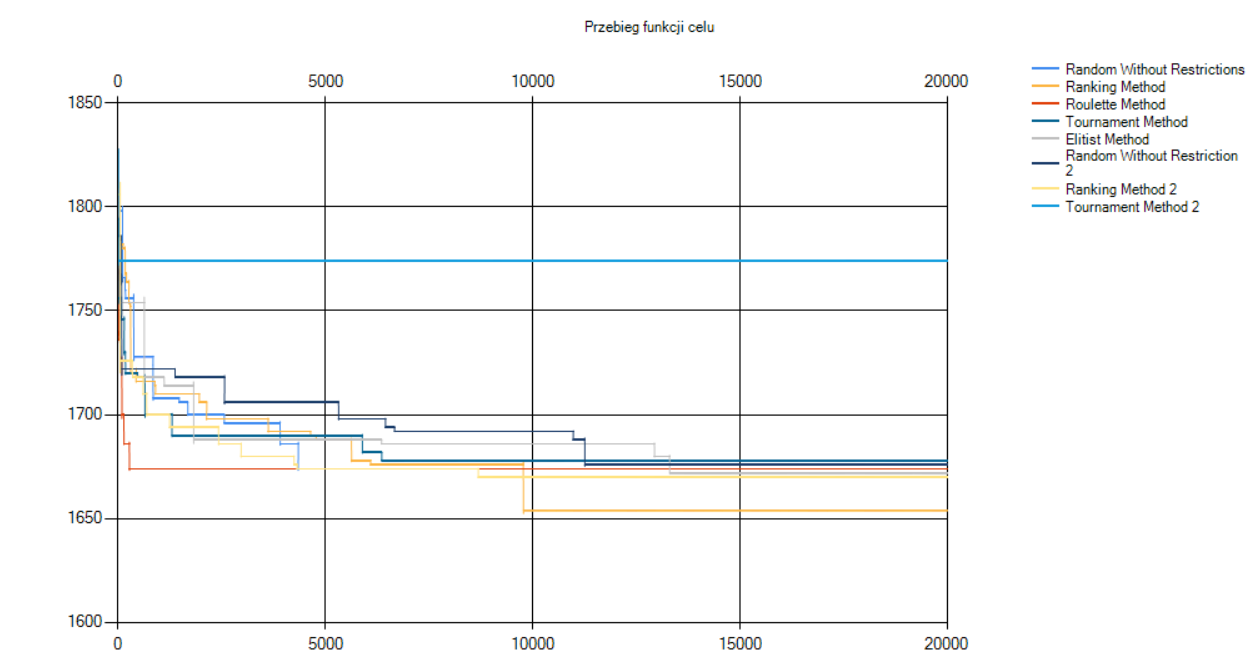
\includegraphics[scale=0.6]{../../../../Screeny/matody_1654_legend.png}
		\caption{Przebiej działania algorytmu dla poszczególnych metod selekcji}
		\label{ranking}			
\end{figure}

Na podstawie tabeli \ref{instancja1} zauważalne staje się zmniejszanie wartości funkcji celu w kolejnych iteracjach algorytmu.  W przypadku metod takich jak metoda ruletki czy też metoda turniejowa, która dopuszcza powtórzeń wśrod osobników w grupie rodzicielskiej, stabilizacja poziomu następuje w początkowych iteracjach i utrzymuje się tak do końca. Powodem tak szybkiej zbieżności tych metod jest brak różnorodności w kolejnych grupach rodzicielskich. W metodzie ruletki spowodowane jest to dużym prawdopodobieństwem wylosowania osobnika najlepszego co prowadzi do jego dominanty nad innymi. Natomiast w metodzie  turniejowej turniej jest w większości przypadków wygrywany przez ten sam osobnik, co przy dodatkowym założeniu iż w jednej grupie rodzicielskiej mogą znajdować się te same osobniki prowadzi do sytuacji że na grupę rodzicielską składają się 3 te same osobniki. Pomimo wrażenia iż rozwiązania osiągnęły stan stabilny już w 20 000 itreracji, należy sprawdzić czy nie nastąpi jeszcze spadek wartości funkcji celu gdy liczba iteracji zostanie zwiększona. W tym celu ponowione zostają badania metod dla 50 000 iteracji.\\

\subsubsection{50 000 iteracji}

 W tabeli \ref{instancja2} zostały zestawione wartości błedu względnego funkcji celu w kolejnych iteracjach dla poszczególnych metod. W tym przypadku zwiększona została liczba iteracji działania algorytmu dla każdej z metod z 20 000 na 50 000. 

\begin{table}[h!]
\begin{center}
\scalebox{0.6}{
\begin{tabular}{|c|c|c|c|c|c|c|c|c|}
\hline
\textbf{Iteracja}  &\textbf{Losowa}  & \textbf{Rankingowa} & \textbf{Ruletka} & \textbf{Turniejowa} & \textbf{Elitarna} & \textbf{Losowa 2} & \textbf{Rankingowa 2} & \textbf{Turniejowa 2}\\
\hline
 \textbf{1}&2,3 \%&0,6\%&4,47\%&0,24\%&1,21\%&2,66\%&1,93\%&4,6\% \\
\hline
 \textbf{2}&1,93\%&0,6\%&2,05\%&0,6\%&1,33\%&1,45\%&2,42\%&4,47\% \\
\hline
 \textbf{3}&0,24\%&1,81\%&1,93\%&1,33\%&1,93\%&1,21\%&1,21\%&6,29\%  \\
\hline
 \textbf{4}&3,99\%&0,24\%&1,81\%&1,21\%&1,45\%&2,42\%&0,48\%&7,99\%  \\
\hline
 \textbf{5}&2,3\%&0,6\%&1,21\%&0,96\%&2,05\%&4,47\%&1,45\%&8,35\%  \\
\hline
 \textbf{6}&1,69\%&0,48\%&4,47\%&2,3\%&1,45\%&2,54\%&1,21\%&9,2\%\\
\hline
 \textbf{7}&1,33\%&0,24\%&1,93\%&0,6\%&1,45\%&1,21\%&1,08\%&7,26\% \\
\hline
 \textbf{8}&2,42\%&0,84\%&1,81\%&0,96\%&0,72\%&1,39\%&2,05\%&6,77\%\\
\hline
 \textbf{9}&0,84\%&\color{green}\textbf{0\%}&0,6\%&0,72\%&1,08\%&2,05\%&2,42\%&8,83\%\\
\hline
 \textbf{10}&2,54\%&0,48\%&2,78\%&0,72\%&2,78\%&1,93\%&2,66\%&5,69\%\\
\hline
 \textbf{11}&2,54\%&0,24\%&1,69\%&1,33\%&1,45\%&3,14\%&3,14\%&3,87\%\\
\hline
 \textbf{12}&0,6 \%&0,48\%&2,05\%&0,48\%&0,6\%&2,66\%&0,96\%&10,53\%\\
\hline
 \textbf{13}&1,33\%&0,84\%&3,14\%&1,08\%&1,21\%&2,66\%&1,45\%&8,59\%\\
\hline
 \textbf{14}&0,84\%&0,24\%&2,3\%&1,45\%&1,21\%&4,47\%&1,21\%&5,69\%\\
\hline
 \textbf{15}&2,54\%&1,45\%&1,33\%&0,6\%&2,3\%&3,63\%&1,81\%&6,29\%\\
\hline
 \textbf{16}&1,08\%&0,6\%&2,66\%&0,96\%&1,81\%&1,45\%&1,08\%&10,53\%\\
\hline
 \textbf{17}&1,81\%&\color{green}\textbf{0\%}&1,33\%&0,72\%&1,21\%&3,99\%&0,48\%&9,2\%\\
\hline
 \textbf{18}&1,57\%&0,48\%&3,26\%&1,93\%&1,93\%&2,17\%&1,45\%&7,14\%\\
\hline
 \textbf{19}&1,08\%&0,48\%&1,57\%&0,84\%&2,3\%&3,99\%&0,96\%&6,53\%\\
\hline
 \textbf{20}&1,93\%&0,6\%&3,14\%&2,42\%&2,05\%&1,45\%&1,93\%&10,53\%\\
\hline
 \textbf{ŚREDNIA}&1,75\%&0,57\%&2,4\%&1,08\%&1,47\%&2,55\%&1,57\%&7,42\%\\
\hline
 \textbf{ODCHYLENIE STANDARDOWE}&0,85\%&0,42\%&0,93\%&0,57\%&0,51\%&1,06\%&0,7\%&1,99\%\\
\hline
\end{tabular}}
\caption{Wartości błędu względnego funkcji celu dla poszczególnych metod selekcji}
\label{instancja2}
\end{center}
\end{table}

W przypadku 50 000 iteracji zauważalne jest uzyskiwanie lepszych średnich wyników przez metody takie jak : metoda rankingowa, metoda elitarna oraz turniejowa dopuszczające istnienie powtorzeń w grupie rodzicielskiej. Dzieje się tak za przyczyną faktu, iż metody te nie kończą stabilizacji funkcji celu na poziomie 20 000, ponieważ następuje spadek wartośći funkcji celu również w dalszych iteracjach. Pozostałe metody utrzymały średnią na tym samym bądź też nieco wyższym poziomie w stosunku to próby testowej zakładającej 20 000 iteracji. Poniżej w tabeli \ref{ranking2} zestawiony został ranking metod uporządkowany od metody działającej najlepiej na pierwszym miejscu do metody działającej najmniej korzystnie na ostatnim.

\begin{table}[h!]
\begin{center}
\scalebox{0.8}{
\begin{tabular}{|c|c|c|c|}
\hline
\textbf{Miejsce}  &\textbf{Metoda}  & \textbf{Funkcja celu} & \textbf{Ilość wygranych}\\
\hline
 \textbf{1}&Rankingowa&0,57\%& 15\\
\hline
 \textbf{2}&Turniejowa&1,08\%& 3\\
\hline
 \textbf{3}&Elitarna&1,47\%& 1\\
\hline
 \textbf{4}&Rankingowa 2&1,57\%& 0\\
\hline
 \textbf{5}&Losowa&1,75\%& 1\\
\hline
 \textbf{6}&Ruletki&2,4\%& 0\\
\hline
 \textbf{7}&Losowa 2&2,55\%& 0\\
\hline
 \textbf{8}&Turniejowa 2&7,42\%& 0\\
\hline
\end{tabular}}
\caption{Ranking metod selekcji na podstawie średniej wartości błędu względnego funkcji celu}
\label{ranking2}
\end{center}
\end{table}

Na podstawie tabeli \ref{ranking2} można wysunąc wniosek iż po raz kolejny nalepsze wyniki uzyskuje metoda rankingowa, a zaraz po niej po raz kolejny najbardziej korzystnie zachowuje się metoda turniejowa. Nie mniej jednak przodowanie tych metod może mieć miejsce w przypadku założonej instancji danych wejściowych, dlatego należy przeprowadzić testy przy użyciu innej macierzy odległości oraz  przepływu. Przebieg funkcji celu we wszystkich 50000 iteracjach widoczny jest na wykresie \ref{ranking2pic}. Konkretnie w przypadku wykresu \ref{ranking2pic} nie istnieją zmiany wartości funkcji po przekroczeniu bariery 20000 iteracji. Jednak analizujac wykres \ref{ranking2picun} widoczny jest spadek dla metody turniejowej w której istnieje zastrzeżenie co do niepowtarzalności się osoników w grupie rozrodczej.

\begin{figure}[h!]
		\includegraphics[scale=0.6]{../../../../Screeny/najlepsze_1652.png}
		\caption{Przebiej działania algorytmu dla poszczególnych metod selekcji}
		\label{ranking2pic}			
\end{figure}

\begin{figure}[h!]
		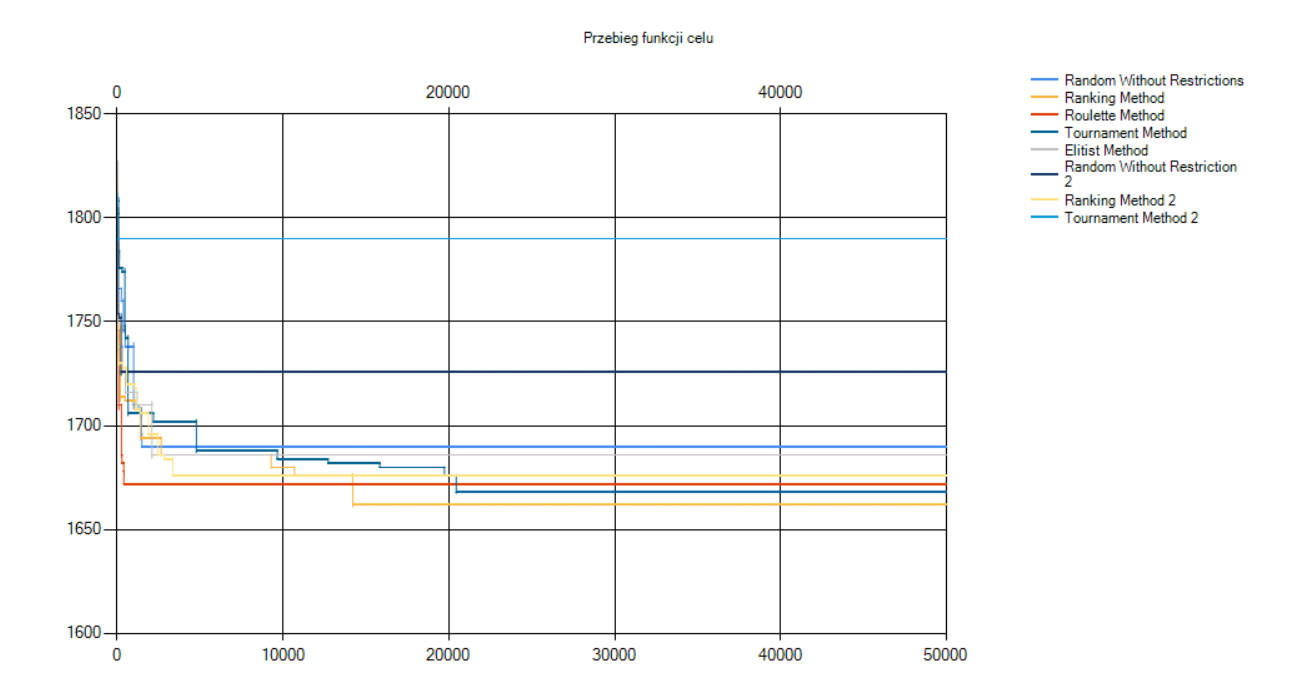
\includegraphics[scale=0.6]{../../../../Screeny/50_tys.png}
		\caption{Przebiej działania algorytmu dla poszczególnych metod selekcji}
		\label{ranking2picun}			
\end{figure}

Analizując powyższe wykresy możliwe jest ustalenie optymalnej ilości iteracji na liczbę 30 000, wówczas wartości funkcji celu w poszczególnych metodach osiągną już stan stabilny, a dodatkowe obliczenia dla liczby równej aż 50 000 iteracji nie bądą musiały być wykonywane.

\subsection{Dane wejściowe instancja II}

\par
$$
\mathbf{Macierz\_przepływu} =
\left( \begin{array}{cccccccccccccccccc}
0& 1& 2& 2& 3& 4& 4& 5& 3& 5& 6& 7& 8& 9& 7& 8& 4& 5\\
1& 0& 1& 1& 2& 3& 3& 4& 2& 4& 5& 6& 7& 8& 6& 7& 3& 4\\
2& 1& 0& 2& 1& 2& 2& 3& 1& 3& 4& 5& 6& 7& 5& 6& 2& 3\\
2& 1& 2& 0& 1& 2& 2& 3& 3& 3& 4& 5& 6& 7& 5& 6& 4& 5\\
3& 2& 1& 1& 0& 1& 1& 2& 2& 2& 3& 4& 5& 6& 4& 5& 3& 4\\
4& 3& 2& 2& 1& 0& 2& 3& 3& 1& 2& 3& 4& 5& 3& 4& 4& 5\\
4& 3& 2& 2& 1& 2& 0& 1& 3& 1& 2& 3& 4& 5& 3& 4& 4& 5\\
5& 4& 3& 3& 2& 3& 1& 0& 4& 2& 1& 2& 3& 4& 2& 3& 5& 6\\
3& 2& 1& 3& 2& 3& 3& 4& 0& 4& 5& 6& 7& 8& 6& 7& 1& 2\\
5& 4& 3& 3& 2& 1& 1& 2& 4& 0& 1& 2& 3& 4& 2& 3& 5& 6\\
6& 5& 4& 4& 3& 2& 2& 1& 5& 1& 0& 1& 2& 3& 1& 2& 6& 7\\
7& 6& 5& 5& 4& 3& 3& 2& 6& 2& 1& 0& 1& 2& 2& 3& 7& 8\\
8& 7& 6& 6& 5& 4& 4& 3& 7& 3& 2& 1& 0& 1& 1& 2& 8& 9\\
9& 8& 7& 7& 6& 5& 5& 4& 8& 4& 3& 2& 1& 0& 2& 1& 9& 10\\
7& 6& 5& 5& 4& 3& 3& 2& 6& 2& 1& 2& 1& 2& 0& 1& 7& 8\\
8& 7& 6& 6& 5& 4& 4& 3& 7& 3& 2& 3& 2& 1& 1& 0& 8& 9\\
4& 3& 2& 4& 3& 4& 4& 5& 1& 5& 6& 7& 8& 9& 7& 8& 0& 1\\
5& 4& 3& 5& 4& 5& 5& 6& 2& 6& 7& 8& 9& 10& 8& 9& 1& 0\\
\end{array} \right)
$$

\par
$$
\mathbf{Macierz\_odległości} =
\left( \begin{array}{cccccccccccccccccc}
   0& 3& 4& 6& 8& 5& 6& 6& 5& 1& 4& 6& 1& 5& 4& 5& 6& 8\\
    3& 0& 6& 3& 7& 9& 9& 2& 2& 7& 4& 7& 9& 6& 3& 2& 6& 6\\
    4& 6& 0& 2& 6& 4& 4& 4& 2& 6& 3& 6& 5& 6& 2& 6& 5& 7\\
    6& 3& 2& 0& 5& 5& 3& 3& 9& 4& 3& 6& 3& 4& 7& 8& 3& 2\\
    8& 7& 6& 5& 0& 4& 3& 4& 5& 7& 6& 7& 7& 3& 3& 3& 4& 4\\
    5& 9& 4& 5& 4& 0& 8& 5& 5& 5& 7& 5& 1& 8& 5& 4& 3& 3\\
    6& 9& 4& 3& 3& 8& 0& 6& 8& 4& 6& 7& 1& 8& 5& 6& 7& 6\\
    6& 2& 4& 3& 4& 5& 6& 0& 1& 5& 5& 3& 7& 5& 9& 4& 4& 4\\
    5& 2& 2& 9& 5& 5& 8& 1& 0& 4& 5& 2& 4& 5& 4& 5& 4& 7\\
    1& 7& 6& 4& 7& 5& 4& 5& 4& 0& 7& 7& 5& 6& 5& 5& 6& 10\\
    4& 4& 3& 3& 6& 7& 6& 5& 5& 7& 0& 9& 6& 5& 1& 8& 5& 3\\
    6& 7& 6& 6& 7& 5& 7& 3& 2& 7& 9& 0& 6& 5& 4& 5& 4& 6\\
    1& 9& 5& 3& 7& 1& 1& 7& 4& 5& 6& 6& 0& 5& 7& 4& 5& 2\\
    5& 6& 6& 4& 3& 8& 8& 5& 5& 6& 5& 5& 5& 0& 5& 3& 2& 4\\
    4& 3& 2& 7& 3& 5& 5& 9& 4& 5& 1& 4& 7& 5& 0& 8& 5& 6\\
    5& 2& 6& 8& 3& 4& 6& 4& 5& 5& 8& 5& 4& 3& 8& 0& 6& 8\\
    6& 6& 5& 3& 4& 3& 7& 4& 4& 6& 5& 4& 5& 2& 5& 6& 0& 3\\
    8& 6& 7& 2& 4& 3& 6& 4& 7& 10& 3& 6& 2& 4& 6& 8& 3& 0\\
\end{array} \right)
$$

\par

\section{Metody mutacji}\label{sec:strukturaDokumentu}

Testy metod mutacji  w obrębie jednej instancji danych zostały przeprowadzone przy założeniu stałych:
\begin{itemize}
\item
macierzy odległości i macierzy przepływu,
\item
metod reprodukcji,
\item
metoda krzyżowania,
\item
ilość iteracji algorytmu
\end{itemize}
\par
W klasycznych metodach mutacji stosowany jest wybór osobników do grupy rozrodczej poprzez metode losową. Niemniej jednak ze względu na wyjątkowo dobre wyniki uzyskiwane przez metode rankingową w testach przeprowadzanych w rozdziale 7.1, postanowiono sprawdzić jej działanie w połączeniu z różnymi wariantami metod mutacji. Ilość iteracji algorytmu była równa, podobnie jak w powyższych testach, 20 000 iteracji, a następnie, w celu zbadania czy w dalszych niż granica 20 000 następuje spadek wartości funkcji celu, również dla 50 000 iteracji. Zgodnie z podrozdziałem 4.2.4 metody mutacji zostaną dodatkowo przetestowane pod kątem wpływu na ich działanie parametru $\leftthreetimes$.

\subsection{Dane wejściowe instancja I}
Dane wejściowe, określające macierz odległości i macierz przepywu, umieszczone zostały w rozdziale 7.1.1 oraz 7.1.2.
\subsubsection{Reprodukcja losowa}

\begin{table}[h!]
\begin{center}
\scalebox{0.55}{
\begin{tabular}{|c|c|c|c|c|c|c|c|c|}
\hline
\textbf{Iteracja}  &\textbf{DE/rand/1}  & \textbf{DE/rand/1+$\leftthreetimes$} & \textbf{DE/best/1} & \textbf{DE/best/1+$\leftthreetimes$} & \textbf{DE/rand/$n_{v}$} & \textbf{DE/rand/$n_{v}$+$\leftthreetimes$} & \textbf{ DE/current to best/$n_{v}+1$} & \textbf{ DE/current to best/$n_{v}+1$+$\leftthreetimes$}\\
\hline
 \textbf{1}&0,84 \%&0,72\%&1,21\%&1,33\%&0,6\%&0,24\%&0,48\%&0,24\% \\
\hline
 \textbf{2}&1,08\%&0,24\%&1,81\%&1,08\%&0,72\%&0,48\%&0,6\%&0,24\% \\
\hline
 \textbf{3}&0,48\%&0,24\%&2,05\%&2,54\%&0,72\%&0,48\%&0,24\%&0,84\%  \\
\hline
 \textbf{4}&0,48\%&0,24\%&1,33\%&0,48\%&0,24\%&0,48\%&0,48\%&0,48\%  \\
\hline
 \textbf{5}&0,72\%&0,72\%&0,48\%&0,48\%&0,6\%&0,24\%&0,48\%&0,24\%  \\
\hline
 \textbf{6}&1,08\%&0,84\%&2,78\%&1,21\%&0,48\%&0,6\%&0,48\%&0,24\%\\
\hline
 \textbf{7}&0,84\%&0,48\%&1,33\%&1,21\%&0,84\%&0,48\%&1,21\%&0,24\% \\
\hline
 \textbf{8}&1,21\%&0,48\%&0,48\%&1,57\%&1,81\%&0,24\%&0,48\%&0,24\%\\
\hline
 \textbf{9}&0,24\%&0,6\%&1,21\%&1,57\%&0,84\%&1,08\%&0,84\%&0,48\%\\
\hline
 \textbf{10}&1,33\%&0,72\%&1,33\%&1,21\%&1,08\%&0,48\%&\color{green}\textbf{0\%}&0,6\%\\
\hline
 \textbf{11}&0,84\%&\color{green}\textbf{0\%}&0,84\%&1,33\%&0,12\%&0,12\%&\color{green}\textbf{0\%}&1,08\%\\
\hline
 \textbf{12}&0,24\%&0,48\%&1,69\%&1,57\%&0,96\%&0,48\%&0,48\%&\color{green}\textbf{0\%}\\
\hline
 \textbf{13}&0,72\%&0,84\%&0,6\%&1,57\%&0,6\%&0,48\%&1,08\%&0,24\%\\
\hline
 \textbf{14}&0,48\%&0,12\%&0,96\%&1,33\%&0,48\%&0,24\%&0,84\%&1,21\%\\
\hline
 \textbf{15}&\color{green}\textbf{0\%}&0,24\%&0,48\%&0,24\%&1,21\%&0,24\%&\color{green}\textbf{0\%}&\color{green}\textbf{0\%}\\
\hline
 \textbf{16}&0,48\%&0,6\%&2,3\%&1,69\%&0,6\%&0,72\%&\color{green}\textbf{0\%}&0,48\%\\
\hline
 \textbf{17}&0,6\%&0,12\%&2,54\%&2,17\%&0,48\%&0,6\%&0,6\%&0,24\%\\
\hline
 \textbf{18}&1,81\%&0,6\%&2,17\%&1,33\%&0,48\%&0,48\%&0,6\%&0,48\%\\
\hline
 \textbf{19}&1,08\%&0,24\%&1,21\%&1,21\%&1,57\%&0,48\%&0,48\%&0,6\%\\
\hline
 \textbf{20}&0,72\%&0,6\%&2,66\%&0,84\%&0,48\%&0,48\%&0,48\%&0,72\%\\
\hline
 \textbf{ŚREDNIA}&0,77\%&0,46\%&1,48\%&1,31\%&0,75\%&0,46\%&0,44\%&0,45\%\\
\hline
 \textbf{ODCHYLENIE}&0,41\%&0,25\%&0,73\%&0,49\%&0,41\%&0,21\%&0,3\%&0,32\%\\
\hline
\end{tabular}}
\caption{Wartości błędu względnego funkcji celu dla poszczególnych metod mutacji}
\label{losowa20}
\end{center}
\end{table}
\par
Analizując tabele \ref{losowa20} widoczny staje się fakt iż, najlepsze wyniki uzyskiwane są dla strategii \textbf{DE/current to best/\textbf{$n_{v}+1$}} jako, że aż 4 razy algorytm z udziałem tej metody mutacji osiągał błąd względy równy 0\%. W pozostałych iteracjach wartości błedu względnego w przeważajacej części również były niewielkie, rzędu 0 - 0,48\%.  Współczynnik  odchylenia standardowego dla wspomnianej powyżej metody jest równy 0,3 \%, co świadczy o bliskim skupieniu wartości w poszczególnych iteracjach wokół średniej. Jest to również jedna z mniejszych wartości odchylenia standardowego biorąc pod uwagę inne metody mutacji.\\
Strategia  DE/current to best/$n_{v}+1$ z uwzględnieniem zależności opisanych w podrozdziale 4.2.4, a więc z wprowadzeniem dodatkowego współczynnika $\leftthreetimes$, również przynosi satysfakcjonujące wyniki. Średni błąd względny wynosi 0,45\%, a algorytm 2 razy doprowadza funkcję celu do wartości uznawanej przez \cite{qaplib} za najmniejszą znaną wartość. W tabeli \ref{ranking3} został przedstawiony ranking metod mutacji ułożony w zależności od uzyskanej przez metody te średniej wartości błędu wzglednego.

\begin{table}[h!]
\begin{center}
\scalebox{0.8}{
\begin{tabular}{|c|c|c|c|}
\hline
\textbf{Miejsce}  &\textbf{Metoda}  & \textbf{Funkcja celu} & \textbf{Ilość wygranych}\\
\hline
 \textbf{1}&DE/current to best/$n_{v}+1$&0,44\%& 7\\
\hline
 \textbf{2}& DE/current to best/$n_{v}+1$+$\leftthreetimes$&0,45\%& 9\\
\hline
 \textbf{3}&DE/rand/$n_{v}$+$\leftthreetimes$&0,46\%& 5\\
\hline
 \textbf{4}&DE/rand/1+$\leftthreetimes$&0,46\%& 7\\
\hline
 \textbf{5}&DE/rand/$n_{v}$&0,75\%&3\\
\hline
 \textbf{6}&DE/rand/1&0,77\%& 2\\
\hline
 \textbf{7}&DE/best/1+$\leftthreetimes$&1,32\%& 0\\
\hline
 \textbf{8}&DE/best/1&1,48\%& 0\\
\hline
\end{tabular}}
\caption{Ranking metod mutacji na podstawie średniej wartości błędu względnego funkcji celu}
\label{ranking3}
\end{center}
\end{table}

Na podstawie tabeli \ref{ranking3} można wysnuć wniosek, iż metody takie jak  DE/current to best/$n_{v}+1$+$\leftthreetimes$, DE/rand/1+$\leftthreetimes$ oraz  DE/best/1+$\leftthreetimes$, a wiec metody które zostały zmodyfikowane współczynnikiem $\leftthreetimes$ uzyskują korzystniejsze wyniki w porównaniu do ich odpowiedników bez modyfikatora. Widoczna staje się zatem skuteczność działania czynnika skalującego $\leftthreetimes$.














